\section{{\tool}: Approach Overview}
\label{overview:sec}

%{\tool} has two main processes: training and predicting.


\subsection{Training Process}

Figure~\ref{overview-training} shows the overview of our training
process. If a method has multiple buggy statements, we treat one buggy
statement and~its enclosing method at a time as a training
instance. The input of~this process is the source code of a buggy
method and one of its buggy statements, and the respective fixed
source code.  The output includes the trained tree-based CCL model and
the trained tree-based CTL model.
%
%code context learning model (CCL model to learn the surrounding code
%context) and the trained tree-based code transformation learning model
%(CTL model to learn the bug-fixing code transformations) with their
%parameters.
The training process has two main steps:

\begin{figure}[t]
	\centering
	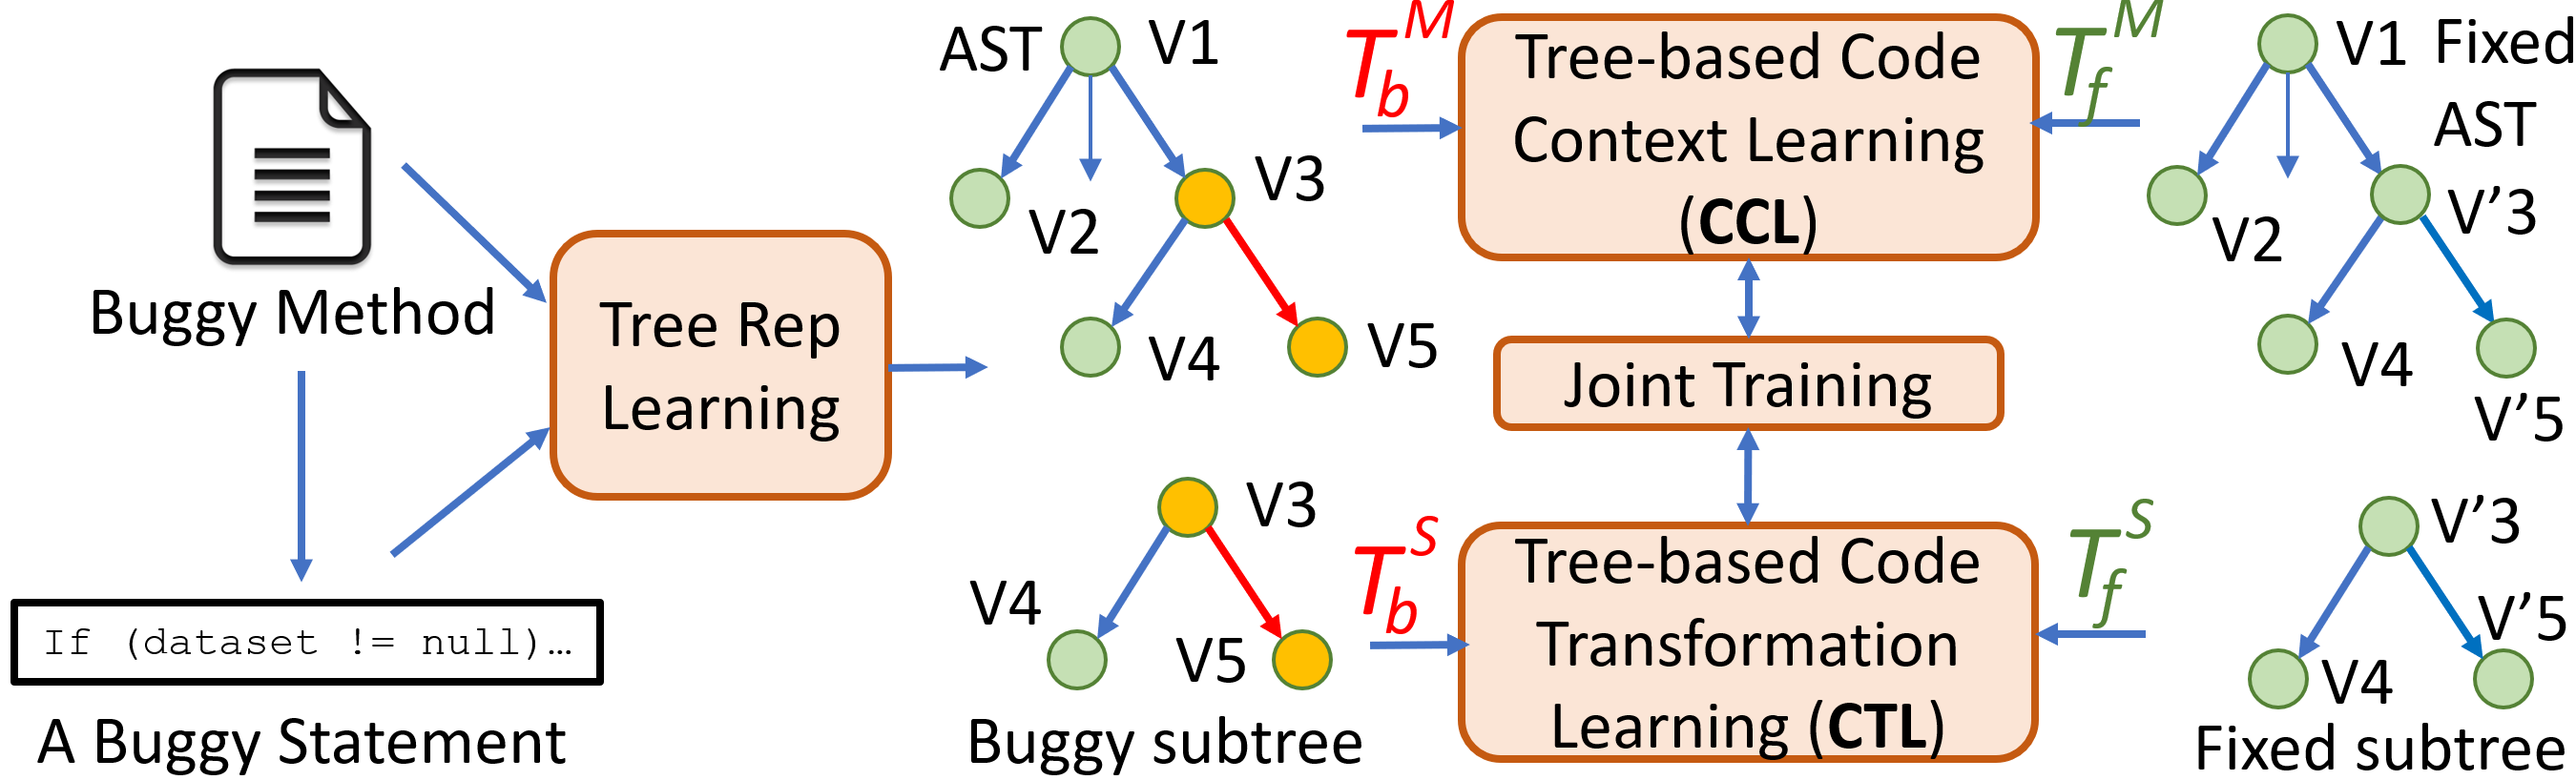
\includegraphics[width=3.4in]{graphs/new_overview-2.png}
        \vspace{-15pt}
	\caption{{\tool}: Training Process}
	\label{overview-training}
%	\vspace{-10pt}
\end{figure}

%\vspace{3pt}
\noindent {\bf Tree-based Representation Learning.} This step aims to
take the source code and to build the tree-based vector
representations (embeddings) to be the inputs of CCL and CTL. To
achieve that, the given method is parsed to obtain its AST
and the subtree for the buggy statement.
%we first parse the given source code to obtain the AST for the given
%method and the subtree for the buggy statement.
Then, the word embedding technique, GloVe~\cite{pennington2014glove},
is used to produce the vector for each node in the AST when we flatten
the AST into a sequence. The output of this step is the AST for the
method and the AST subtree for the buggy statement
in which each node is replaced by its embedding vector
(Figure~\ref{overview-training}).

\vspace{3pt}
\noindent {\bf Context-aware, Dual-Task Learning Automated Program
  Repair.}  The goal of this step is to train both of the tree-based
CCL and the tree-based CTL in a joint-training manner. The entire AST
$T^{M}_b$ of the buggy method after vectorization (i.e., each node is
a vector) is used at the input layer of CCL for training. The AST of
the corresponding fixed method $T^{M}_f$ after vectorization is used
at the output layer of the CCL model. Similarly, the AST subtree
$T^{S}_b$ of the buggy statement after vectorization is used at the
input layer of CTL, and the subtree $T^{S}_f$ of the fixed statement
after vectorization is used at the output layer of the CTL model. Each
of the CCL and CTL models is realized via an attention-based
\code{seq2seq} model.
%Instead of cascading the two models CCL and CTL,
We use the {\em cross-stitch unit}~\cite{misra2016cross} to train CCL
and CTL simultaneously with soft-sharing the parameters to exploit
this duality. Joint training is aimed to learn the shared
representations between CCL amd CTL in terms of a linear combination
of the input features in both models. The output of this step includes
the trained CCL and CTL models.

\subsection{Prediction Process}



Figure~\ref{overview-fixing} illustrates the prediction process, i.e.,
the automated fixing process. A common usage of our tool is that
before using it, a developer could use a fault localization tool
(FL) to detect a buggy statement that needs to be fixed. Then, the
input for APR is the buggy statement in the enclosing method.
%Another usage is that a developer can pinpoint the buggy statement and
%invoke {\tool} for an auto-fixing suggestion.
The fixing process shares the first step of Tree-based Representation
Learning with the training process. After that step, the vectorized
buggy AST subtree (each tree node is represented by a vector), is used
as the input of the {\em trained tree-based} CTL. The output of the
trained CTL model is the fixed AST subtree, which is converted back
into source code to form a candidate patch. We design a novel patch
generation that uses beam search over the AST structure and works in
accordance with the decoder as part of CTL in order to improve
efficiency. Finally, we adopt the patch validation process via test
cases as in DLFix~\cite{icse20}.

%the candidate patches are validated and output.

%We design a novel patch validation scheme that makes use of beam
%search for an efficient process. The final candidate patches are then
%produced.

\begin{figure}[t]
	\centering
	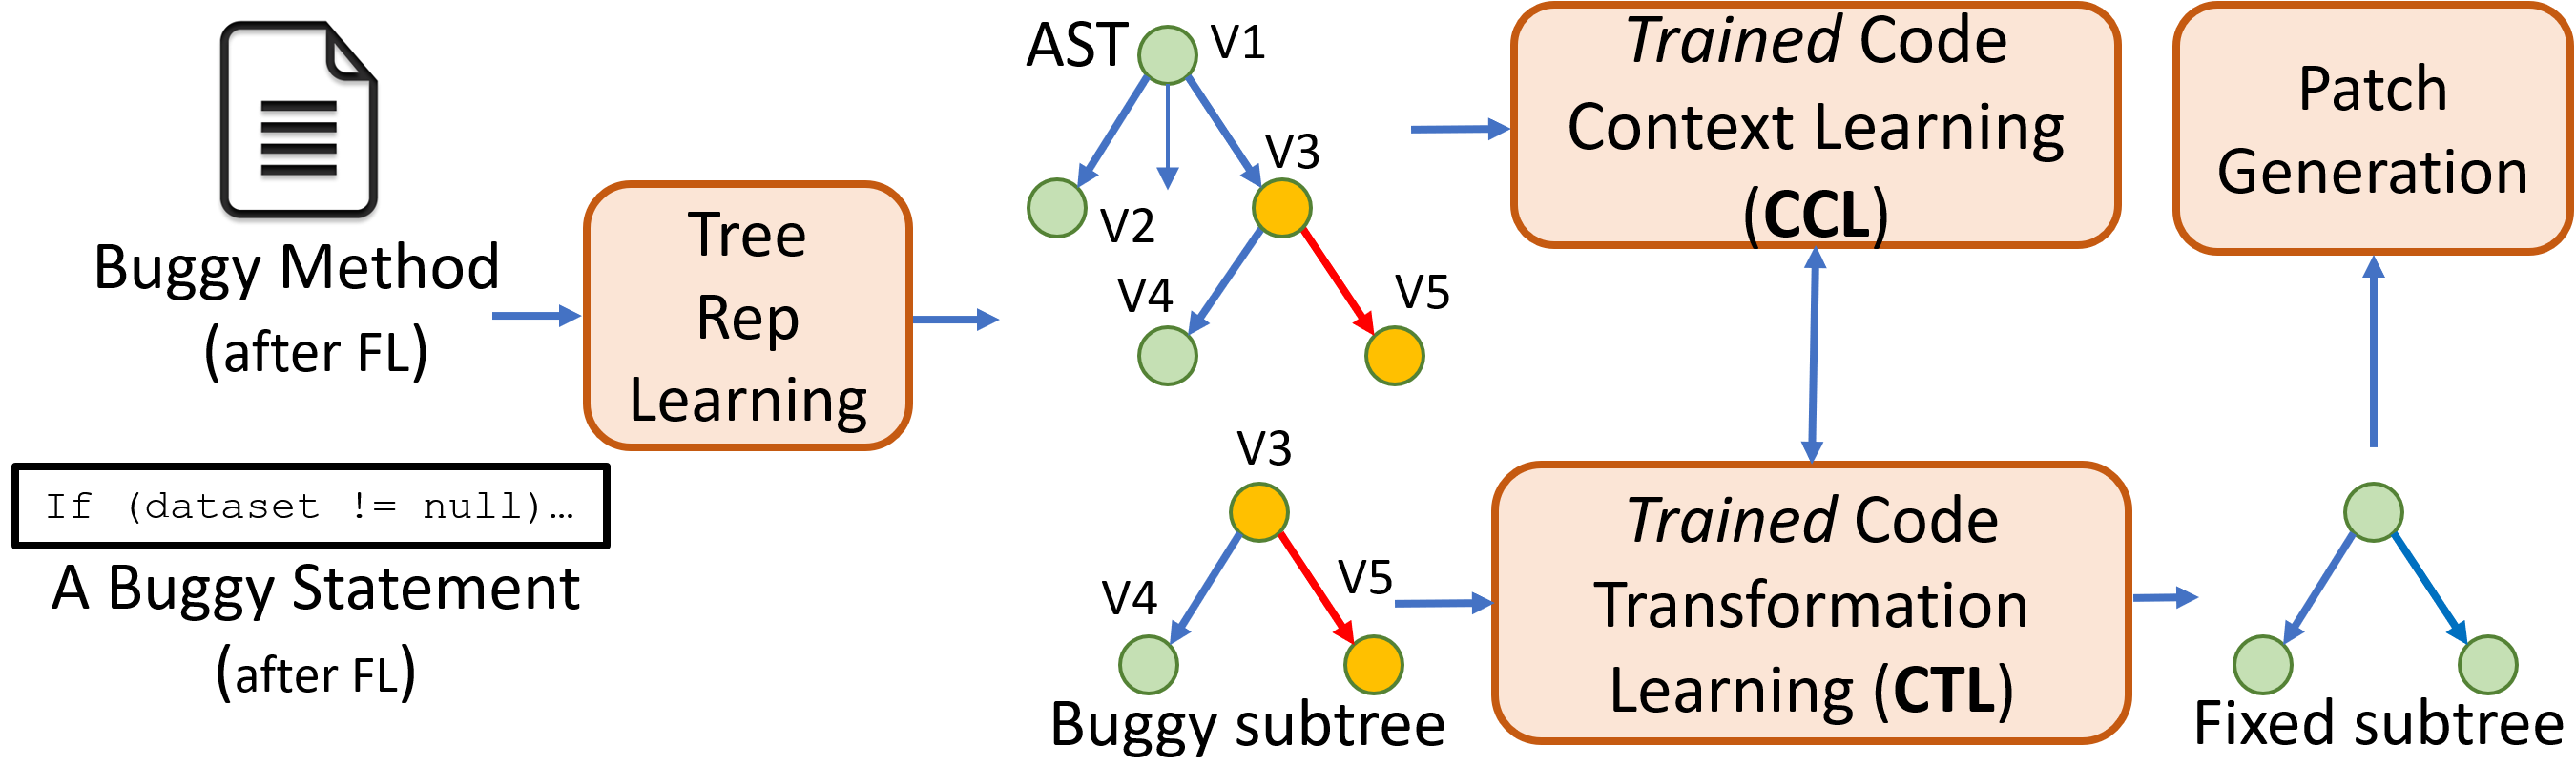
\includegraphics[width=3.4in]{graphs/overview-predict-2.png}
	\caption{{\tool}: Fixing Process}
        \vspace{-3pt}
	\label{overview-fixing}
\end{figure}
